\setstretch{2}
%\setlength{\parindent}{3em}
\setlength{\parskip}{1em}

Escribe tu capítulo 2


\section{Añadamos algunas ecuaciones}
\setlength{\parindent}{0em}

Enumera tus ecuaciones

Regresión Lineal (Mínimos Cuadrados Ordinarios)

\begin{equation}
\hat{\beta }=min\sum_{i=1}^{n}\left ( y_i-\beta_0-\sum_{i=1}^{p} \beta _{j}x_{ij} \right )^{2}
\end{equation}

O si quieres no las enumeres

$$\hat{\beta }=min\sum_{i=1}^{n}\left ( y_i-\beta_0-\sum_{i=1}^{p} \beta _{j}x_{ij} \right )^{2}$$

O puedes utilizar tus ecuaciones dentro del texto $\hat{\beta }=min\sum_{i=1}^{n}\left ( y_i-\beta_0-\sum_{i=1}^{p} \beta _{j}x_{ij} \right )^{2}$.

Y si tienes ecuaciones muy largas, las puedes hacer utilizando:

\begin{equation}
\begin{aligned}
Y  = & [\alpha_0+\alpha_1\ (Y-T)-\alpha_2\ R]+[\beta_0+\beta_1 Y-\beta_2 R]+G\\
Y  = & [\alpha_0+\alpha_1\ Y-\alpha_1\ [\gamma_0+\gamma_1\ Y]-\alpha_2 R]+[\beta_0+\beta_1 Y-\beta_2R]+G\\
Y  = &  [\alpha_0+\alpha_1\ \gamma_0+\beta_0\ ]+[\alpha_1-\alpha_1 \gamma_1+\beta_1 ]Y-[\alpha_2+\beta_2]R+G\\
Y  = & \alpha_1-\alpha_1\ \gamma_1+\beta_1\ ]Y=[\alpha_0+\alpha_1 \gamma_0+\beta_0 ]-[\alpha_2+\beta_2 ]R+G\\
Y  = & [1/(1-\alpha_1+\alpha_1\ \gamma_1-\beta_1\ )][(\alpha_0-\alpha_1 \gamma_0+\beta_0)-(\alpha_2+\beta_2)R+G] 
\end{aligned}
\end{equation}

\section{Añadamos unas figuras}


\begin{figure}[h!]
\caption{Pronóstico de crecimiento económico global 2020}
\label{fig:GrowthGDP}
\centering
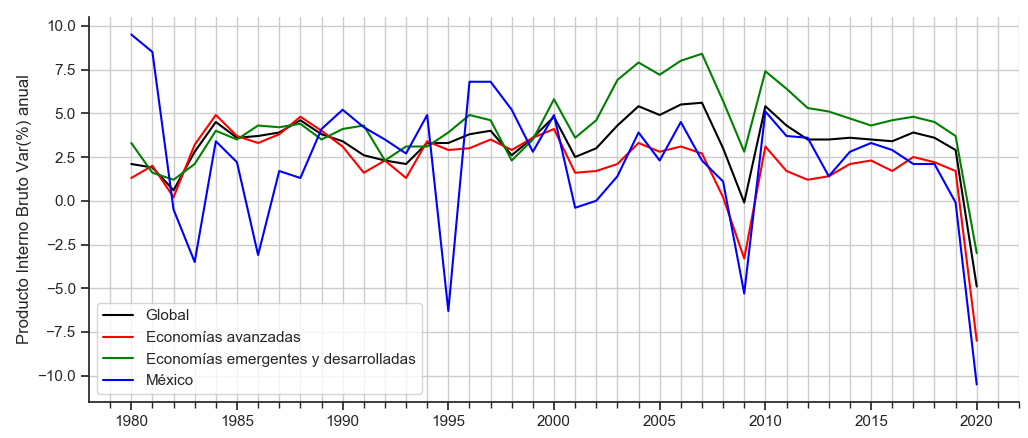
\includegraphics[width=1\textwidth]{Figuras/GDP.png}
\caption*{Fuente: elaboración propia con datos del FMI}
\end{figure}

\newpage
\section{También una tabla}

\begin{table}[h]
\centering
\caption{Comparación de contracciones económicas}
\begin{tabular}{ccccc}
\textbf{Año} &
  \textbf{Mundial} &
  \textbf{\begin{tabular}[c]{@{}c@{}}Economías\\ avanzadas\end{tabular}} &
  \textbf{\begin{tabular}[c]{@{}c@{}}Economías emergentes\\ y desarrolladas\end{tabular}} &
  \textbf{México} \\ \hline
1995     & 3.3  & 2.9  & 3.9  & -6.3  \\
2009     & -0.1 & -3.3 & 2.8  & -5.3  \\
$2020^E$ & -4.9 & -8.0 & -3.0 & -10.5 \\ \hline
\end{tabular}
\begin{tablenotes}
\centering
\item Fuente: elaboración propia con datos del FMI.
\end{tablenotes}
\end{table}

Aquí podemos describir los resultados de la tabla.

\begin{table}[h]
\centering
\caption{Precios de OMA}
\label{tab:OMA}
\begin{tabular}{ll}
\multicolumn{1}{c}{\textbf{Date}} & \multicolumn{1}{c}{\textbf{Close}} \\ \hline
15/04/2016                        & 100.169998                         \\
18/04/2016                        & 99.339996                          \\
19/04/2016                        & 100.699997                         \\
20/04/2016                        & 100.68                             \\
21/04/2016                        & 100.080002                         \\
22/04/2016                        & 101.660004                         \\
25/04/2016                        & 101.690002                         \\
26/04/2016                        & 97.059998                          \\
27/04/2016                        & 99.639999                         
\end{tabular}
\begin{tablenotes}
\centering
\item Fuente: elaboración propia con datos del Yahoo Finance.
\end{tablenotes}
\end{table}
